\def\hsep{3.6cm}
\def\vsep{-0.2cm}

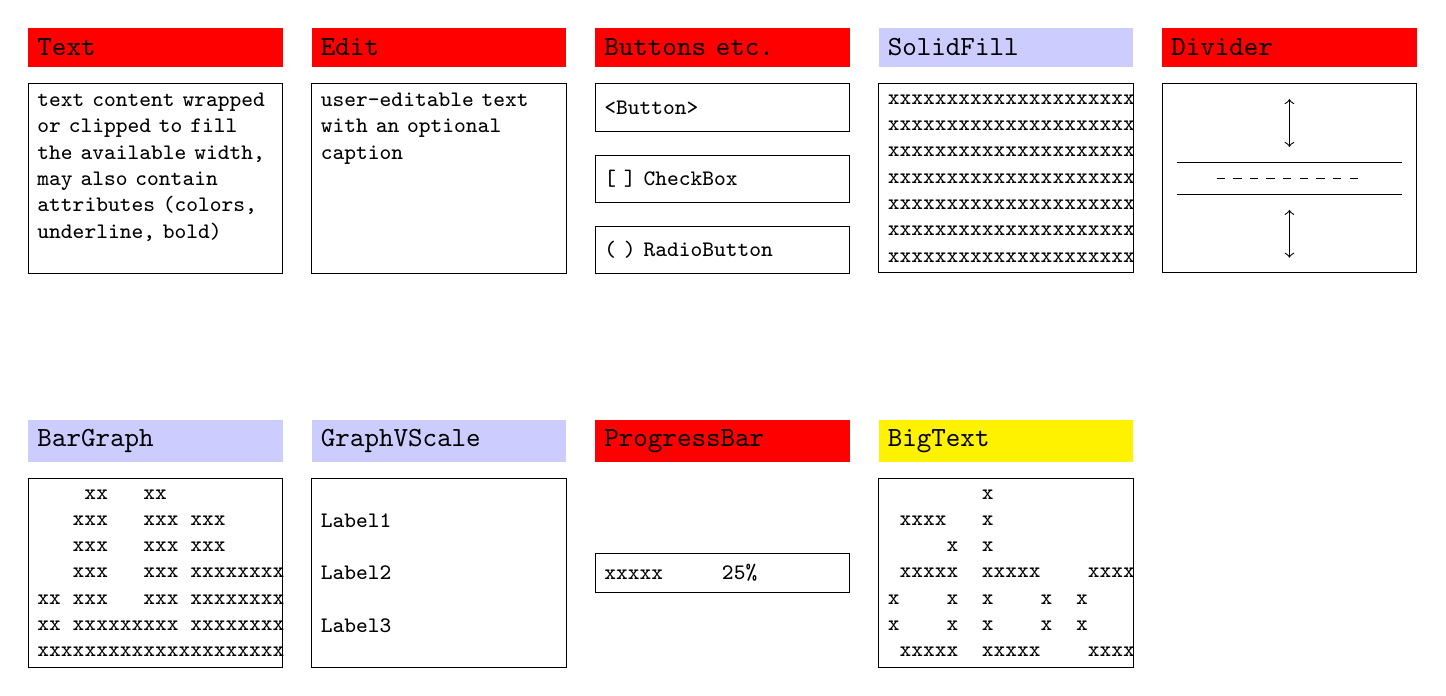
\begin{tikzpicture}[
  all/.style = {fill plain picture = {
    \draw[yellow, line width = 0.9cm] ( 0,-1) -- (2,1);
    \draw[blue!20,   line width = 0.9cm]   (-2,-1) -- (0,1);
    \draw[red,    line width = 0.9cm]   (-1,-1) -- (1,1);
  }},
  box/.style = {fill = blue!20},
  flow/.style = {fill = red},
  fixed/.style = {fill = yellow},
  boxflow/.style = {fill plain picture = {
    \node[fill = blue!20, line width = 0pt, draw = none, minimum size = 4cm, rotate = 45, anchor = south] at (0, 0) {};
    \node[fill = red, line width = 0pt, draw = none, minimum size = 4cm, rotate = 45, anchor = north]  at (0, 0) {};
  }},
  title/.style = {rectangle, minimum width = 3cm, minimum height = 0.5cm, text width = 3cm, align = left, font = \bfseries\ttfamily},
  widget/.style = {title, draw, font = \footnotesize\normalfont\ttfamily},
  blank/.style = {widget, minimum height = 2.4cm},
  shorten >= 0.2cm,
  shorten <= 0.2cm,
]
  \linespread{1}
  \node[title, flow] (text) {Text};
  \node[blank, anchor = north] (text') at ([yshift = \vsep]text.south) {text content wrapped or clipped to fill the available width, may also contain attributes (colors, underline, bold)\\\ };
  
  \node[title, flow] (edit) at ([xshift = \hsep]text) {Edit};
  \node[blank, anchor = north] (edit') at ([yshift = \vsep]edit.south) {user-editable text with an optional caption\\\ \\\ \\\ \\\ };
  
  \node[title, flow] (button) at ([xshift = \hsep]edit) {Buttons etc.};
  \node[blank, anchor = north, minimum height = 0.6cm] (button1) at ([yshift = \vsep]button.south) {  <Button>};
  \node[blank, minimum height = 0.6cm] (button2) at (edit' -| button) {  [ ] CheckBox};
  \node[blank, anchor = south, minimum height = 0.6cm] (button3) at (edit'.south -| button) {  ( ) RadioButton};
  
  \node[title, box] (solidfill) at ([xshift = \hsep]button) {SolidFill};
  \node[blank, anchor = north, align = flush center] (solidfill') at ([yshift = \vsep]solidfill.south) {xxxxxxxxxxxxxxxxxxxxx\\xxxxxxxxxxxxxxxxxxxxx\\xxxxxxxxxxxxxxxxxxxxx\\xxxxxxxxxxxxxxxxxxxxx\\xxxxxxxxxxxxxxxxxxxxx\\xxxxxxxxxxxxxxxxxxxxx\\xxxxxxxxxxxxxxxxxxxxx};
  
  \node[title, flow] (divider) at ([xshift = \hsep]solidfill) {Divider};
  \node[blank, anchor = north, align = flush center] (divider') at ([yshift = \vsep]divider.south) {};
  \draw ([yshift = 0.2cm]divider'.west) -- ([yshift = 0.2cm]divider'.east);
  \draw ([yshift = -0.2cm]divider'.west) -- ([yshift = -0.2cm]divider'.east);
  \draw[dashed] ([xshift = 0.5cm]divider'.west) -- ([xshift = -0.5cm]divider'.east);
  \draw[<->] (divider'.north) -- ([yshift = 0.2cm]divider'.center);
  \draw[<->] (divider'.south) -- ([yshift = -0.2cm]divider'.center);

  \node[title, box] (divider) at ([yshift = -5cm]text) {BarGraph};
  \node[blank, anchor = north, align = flush center] (divider') at ([yshift = \vsep]divider.south) {%
    \begin{minipage}[t]{3cm}
\begin{verbatim}
    xx   xx          
   xxx   xxx xxx     
   xxx   xxx xxx     
   xxx   xxx xxxxxxxx
xx xxx   xxx xxxxxxxx
xx xxxxxxxxx xxxxxxxx
xxxxxxxxxxxxxxxxxxxxx
\end{verbatim}
    \end{minipage}
  };
  
  \node[title, box] (graphvscale) at ([xshift = \hsep]divider) {GraphVScale};
  \node[blank, anchor = north, align = flush left] (graphvscale') at ([yshift = \vsep]graphvscale.south) ;
  
  \node[title, fixed] (bigtext) at ([xshift = \hsep]progressbar) {BigText};
  \node[blank, anchor = north, align = flush center] (bigtext') at ([yshift = \vsep]bigtext.south) {%
  \begin{minipage}[t]{3cm}
\begin{verbatim}
        x            
 xxxx   x            
     x  x            
 xxxxx  xxxxx    xxxx
x    x  x    x  x    
x    x  x    x  x    
 xxxxx  xxxxx    xxxx
\end{verbatim}
  \end{minipage}
  };
\end{tikzpicture}